\documentclass{article}
\usepackage{tikz}
 
\begin{document}

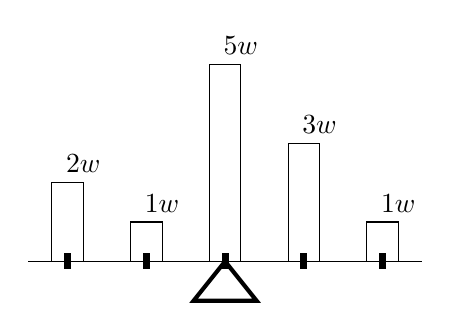
\begin{tikzpicture}

	\draw (-0.5, 0) -- (4.5, 0);
	\foreach \x in {0, 1,...,4} {
		\draw [line width=2.5pt](\x, 0.1) -- (\x, -0.1);
	}

	\coordinate[] (A) at (1.6,-0.5);
	\coordinate[] (B) at (2.4,-0.5);
	\coordinate[] (C) at (2,0);
	\draw [line width=1.5pt] (A) -- (B) -- (C) -- cycle;

	\draw (-0.2, 0) rectangle (0.2, 1);
	\node[above] at (0.2, 1){$2w$};
	\draw (1-0.2, 0) rectangle (1+0.2, 0.5);
	\node[above] at (1+0.2, 0.5){$1w$};
	\draw (2-0.2, 0) rectangle (2+0.2, 2.5);
	\node[above] at (2+0.2, 2.5){$5w$};
	\draw (3-0.2, 0) rectangle (3+0.2, 1.5);
	\node[above] at (3+0.2, 1.5){$3w$};
	\draw (4-0.2, 0) rectangle (4+0.2, 0.5);
	\node[above] at (4+0.2, 0.5){$1w$};
\end{tikzpicture}

\end{document}